\chapter{Background Theory}\label{T-B}
\label{cha:TheoryAndBackground}

This project is a cross-disciplinary one, as it combines machine learning and medicine, and as such, some theory from both disciplines is necessary in order to understand the project. Most of the subsections here were originally found in \citet{forprosjekt}, as the necessary preliminaries are mostly the same as in the specialization project.

\section{Biological Theory}
\label{sec:bio_theory}

The first major part of the theory is the biological/medical part.

\subsection{Lung Cancer}
\label{subsec:lung_cancer}

Lung cancer is the second most common type of cancer worldwide, and the type of cancer with the highest total mortality worldwide, causing about 1.8 million deaths \citep{globalkreftforekomst}. Lung cancer is also the cancer type leading to the most deaths in Norway, amounting to 1500 deaths per year \citep{kreftnorge}. The most important risk factor related to lung cancer is smoking. Smoking is estimated to explain about 90\% of the risk of lung cancer in men, and 70\% to 80\% of the risk of lung cancer in women \citep{roykingrisiko}. Furthermore, about 90\% of lung cancer deaths in men, and 79\% of lung cancer deaths in women are caused by smoking \citep{roykingdod}.

There are two main types of lung cancer, Small Cell Lung Cancers (SCLC) and Non-Small Cell Lung Cancers (NSCLC) \citep{nsclcvsclc}. Of lung cancer cases, about 80-85\% are NSCLC, whilst 10-15\% of the cases are SCLC, and a few percent are minor types of lung cancer \citep{nsclcvsclc2}. NSCLC cancers tend to grow slower than the SCLC cancer types, and thus SCLC has usually already spread when it is diagnosed \citep{nsclcvsclc2}. The NSCLC has three major subtypes: adenocarcinoma (30-40\% of NSCLC cases), squamous cell (30\%) and large-cell undifferentiated carcinoma (10-15\%) \citep{nsclcvsclc}. The treatment and prognosis for the different NSCLC subtypes are similar \citep{nsclcvsclc2}.

Lung cancer develops in different stages. According to \citet{cancerstages}, the main four are:
\begin{enumerate}
    \item The cancer is only situated in your lung
    \item The cancer may have spread to the lymph nodes near the lung
    \item The cancer has spread deeper into the lymph nodes and into the middle of your chest
    \item Cancer is widespread throughout your body
\end{enumerate}

The main advantage of diagnosing lung cancer early is that the cancer has not yet spread to other parts of the body, which means that it can be removed by surgery \citep{cancertreatment}. On the other hand, later stages might require chemotherapy, radiation therapy or immunotherapy, but as the cancer has spread widely, this cure will likely not remove the cancer \citep{cancertreatment}.

%\citet{cancersurvival} found that the 5 year survival reat

\subsection{MicroRNA}

MicroRNAs (miRNAs) are short sequences of RNA, about 22 nucleotides each, that regulate the expression of mRNA by binding to the target mRNA-sequence and thus stopping it from being translated. Circulating miRNA has been found to be a biomarker for many diseases, including cancer, infectious diseases and mental illnesses \citep{mirnabiomarker,mirnabiomarker2,mirnabiomarker3,mirnabiomarker4}. miRNA-sequences are usually named with ``miR'' as prefix and a unique number as suffix. The most commonly used database with known miRNA-sequences is the miRBase database \citep{mirbase}.

\subsection{MicroRNA and Lung Cancer}

The overall role of miRNA in relation to lung cancer is not fully understood \citep{mirnarole}. MicroRNAs are thought to function both as tumor suppressor genes and as oncogenes \citep{mirnarole2}. Multiple studies report differential expression of circulating miRNA-sequences in cancer patients compared to healthy controls, which results in expression of miRNA being a promising method for diagnosing lung cancer \citep{mirnarole}.

\subsection{MicroRNA profiling methods}

There are several methods for measuring levels of miRNA. The most common ones are qRT-PCR, microarrays and sequencing. Here is a very high-level description of the different methods. For more technical details see e.g. \citet{mirnatech}. The different technologies typically have different advantages and disadvantages.

\subsubsection{qRT-PCR}
Quantitative Reverse Transcription - Polymerase Chain Reaction (qRT-PCR) is a common method of measuring miRNA-levels. As the name implies, the process depends on reverse transcription, where miRNA is reverse transcripted, using the enzyme reverse transcriptase, into complementary DNA (cDNA). Then polymerase chain reactions are initiated and monitored in order to measure miRNA-levels.

In qRT-PCR, one needs a primer for each miRNA-sequence that is going to be measured. Therefore, it can only measure miRNA-sequences that are decided beforehand. The main advantage of qRT-PCR is that it is the most sensitive method of the different technologies \citep{mirnatech}, which means that the results are more accurate and that it also works well when the concentration of miRNA is low. 

\subsubsection{Microarrays}
Microarrays are what is called a hybridization method. It starts similarly to qRT-PCR, by converting miRNA into cDNA, but the miRNA is fluorescently labeled in this case. The microarray has several spots, each with single-stranded DNA samples (called probes) that are mounted to the microarray. When the cDNA is added to the microarray, the cDNA will bind to the DNA samples that have the same sequence, in a process called hybridization. Afterward, the microarray is washed clean, and only the cDNA that has managed to bind will remain. Thus, by checking for the fluorescence of the different spots, one can find which DNA-probes had cDNA bind to it, and which had not. The level of fluorescence is then a measure of the concentration of the corresponding miRNA-sequence.

The main advantage of microarrays is that it is the cheapest of the main technologies \citep{mirnatech}. The disadvantages are that it has low sensitivity and that you have to decide beforehand what miRNA-sequences you want to measure, as you need to populate the microarray with the corresponding DNA-probes.  

\subsubsection{Sequencing}
Sequencing also starts with converting miRNA into cDNA. A primer is then connected to the cDNA in one direction. The sequencing step works by adding fluorescent bases one by one, and then see if they add to the sequence starting with the primer. Thus, one can read out the sequence of the cDNA.

The main disadvantage of sequencing is that it is expensive \citep{mirnatech}. It is also less sensitive than qRT-PCR. The main advantage, however, is that you do not need to decide beforehand the miRNA-sequences you want to measure.

\subsection{Types of blood fractions}
\label{met:blood_fluid}

When doing blood profiling, there are different ways to process and filter the blood depending on what parts of the blood one wants in the final sample. There are three different main types.

\subsubsection{Whole blood}
Whole blood is the simplest type, as it is the blood that runs through your body, without any filtering. It might be added anticoagulant, as blood will naturally start clotting outside of the human body unless something is done.

\subsubsection{Serum}
Here you let the blood clot, which means that no anticoagulant is added. When you let the blood clot you end up naturally with a liquid and a solid part, whereas the serum is the liquid part. The solid part has cells, including red blood cells that are thus filtered out. To separate the liquid and solid parts, centrifugation is often used.

\subsubsection{Plasma}
Here you add anticoagulant and then apply centrifugation. Again, the sample will separate into two parts, but here both parts are liquid. The heavy part with all the blood cells will fall to the bottom, and you get a clear liquid at the top. The clear liquid on the top is what is the plasma. One main difference from serum is that plasma contains fibrinogen, which is a protein that is converted to fibrin in blood clotting.

One important thing to note is that serum and plasma are very similar liquids, while whole blood has a different consistency as it contains many cells, especially red blood cells.

\section{Machine learning/statistical theory}
\label{sec:ml_theory}

The second major part of this project is the machine learning.

\subsection{Variance stabilizing transformation}
\label{subsec:var_stab}

In miRNA measurements, one often sees that the variance in miRNA concentration is a function of the mean miRNA concentration. One possible transformation is the log transformation where one takes the logarithm of the data. That can change a curve where $\text{Var}[Y] \propto \text{E}[Y]^2$ into a curve where the variance of $Y$ is independent of the mean of $Y$. One example of this can be seen in \autoref{fig:log_transformation}.

\begin{figure}
    \foreach \time in {Before, After}{
    \begin{subfigure}[b]{0.5\textwidth}
    \resizebox{\textwidth}{!}{
    \begin{tikzpicture}
    \begin{axis}[
        xlabel={Mean miRNA concentration},
        ylabel={Variance of miRNA concentration},
    ]
    \addplot[
        scatter,only marks,scatter src=x,
        table/col sep=comma,
        scatter/use mapped color={draw=blue, fill=blue}
    ]
    table[x=means,y=variances]{tables/VarianceStabilizing/\time.csv};
    \end{axis}
    \end{tikzpicture}
    }
    \caption{\time \ log transformation}
    \label{fig:log_transformation_\time}
    \end{subfigure}
    }
    \caption{Mean and variance in different miRNA-sequences in \citet{Duan2021}}
    \label{fig:log_transformation}
\end{figure}

Another advantage of a variance stabilizing transformation is to ensure that the data is not skewed. Other statistical tools like explained variance (\autoref{subsec:explained_variance}) assume that the underlying data has a normal distribution. A normal distribution, however, has no skew, therefore unskewing the data is necessary for ensuring that other methods are giving valid results. More formally, if we assume that $Y \sim g(X)$ for some function $g$ and that $X \sim N(\mu, \sigma)$, then doing the transformation $y' = g^{-1}(y)$ ensures that our variables are normally distributed. In particular, if we assume that $g(X) = e^{X}$, then the log transformation will ensure that our data is normally distributed. 

\subsection{Fold change}
Fold change is defined as the ratio of a certain value between two different populations. In this project, the fold change used is typically the ratio of levels of a certain miRNA-sequence between cases and controls. Log fold change is the logarithm of the fold change (by convention $\log_2$ is used in this area of research). Furthermore: 

\begin{align*}
    \text{Fold change} &= \frac{a}{b} \\
    \text{Log fold change} &= \log_2 \left(\frac{a}{b}\right) = \log_2 a - \log_2 b
\end{align*}

In other words, the log fold change is the difference in miRNA expression when the data are log transformed.

\subsection{Loess regression}
\label{subsec:loess_regression}

Loess regression is also sometimes called local regression, and it is a type of regression that is made for smoothing scatter plots \citep{loess}. The regression works by fitting a low degree polynomial for each data point. The fitting of each polynomial works by giving weight to nearby points, where more weight is given to points near the original data point. The regression value for each data point is thus the value of the corresponding polynomial evaluated in this point.

Loess regression is practical when the mean and the variance still are not independent after a log transformation. Using loess regression can ensure that they become independent.


\subsection{Principal component analysis}

Principal component analysis (PCA) is a method of data reduction, where a dataset in $\mathbb{R}^n$ is projected down on a lower-dimensional vector space $\mathbb{R}^m$. The projection in PCA is the projection that ensures that most of the variance of the original dataset is kept in the $1 \leq k \leq m$ first principal components, whilst ensuring that the projection is not expanding the dataset. One of the main advantages of PCA is that you could project a dataset down to just two or three dimensions, which makes it possible to plot the dataset.

\subsection{Explained variance}
\label{subsec:explained_variance}

Explained variance is a way of analyzing the sources of variance in a dataset. Using linear regression, one assumes that the dependent variable $y = [y_1, y_2 \dots y_n]$, covariates $\mathbf{X}$ and residuals $\epsilon \sim N(0, \sigma)$ have the relationship $y = \mathbf{X}\beta + \epsilon$, for some parameter vector $\beta$. Furthermore, let $\bar{y}$ be the mean of the $y$'s, i.e $\bar{y} = \frac{1}{n} \sum_{i=1}^n y_i$.


If one creates a linear regression model of the dataset, one gets a parameter vector $\hat{\beta}$ which is the maximum likelihood estimate of $\beta$, and predictions $\hat{y} = \mathbf{X} \hat{\beta}$ for $y$. Also, define $\mathbf{SST} = \sum_{i=1}^n \left(y_i - \bar{y}\right)^2$ as the total sum of squares, $\mathbf{SSR} = \sum_{i=1}^n \left(\hat{y_i} - \bar{y}\right)^2$ as the sum of squares due to regression and $\mathbf{SSE} = \sum_{i=1}^n \left(y_i - \hat{y_i}\right)^2$ as the sum of the squared estimates of errors. Then we have the following relationship:
$$\mathbf{SST} = \mathbf{SSR} + \mathbf{SSE}$$

The proportion of the empirical variance that can be explained by the covariates is thus
$$R^2 = \frac{\mathbf{SSR}}{\mathbf{SST}}$$



\subsection{Wilcoxon signed-rank test}
\label{subsec:wilcoxon-signed-rank}
Wilcoxon signed-rank test is a statistical test to find the location of a distribution \citep{signed-rank-test,signed-rank-2}. More formally, if $\mathbf{X}_1$ and $\mathbf{X}_2$ are independently distributed with cumulative distribution function $\mathit{F}$, and
$$p = P\left(\frac{1}{2}(\mathbf{X}_1 + \mathbf{X}_2) > 0\right)$$
then the test is testing the null hypothesis $p = \frac{1}{2}$ against the alternative hypothesis $p \not = \frac{1}{2}$. The median of $\frac{1}{2}(\mathbf{X}_1 + \mathbf{X}_2)$ is called the pseudomedian of $\mathit{F}$. $\mathit{F}$ is called symmetric about $\mu$ if $f(\mu + x) = f(\mu - x)$. Furthermore, $\mathit{F}$ is called symmetric if there exists such a $\mu$. If $\mathit{F}$ is symmetric, the median and the pseudomedian are the same. Thus, if $\mathit{F}$ is assumed to be symmetric, the null hypothesis is equivalent to that the median of $\mathit{F}$ is $\mu = 0$, against the alternative hypothesis that $\mu \not = 0$.

If one has pairs $(\mathbf{X}, \mathbf{Y})$ where $\mathbf{X} \sim \mathit{F}_X$ and $\mathbf{Y} \sim \mathit{F}_Y$, with the null hypothesis $\mathit{F}_X = \mathit{F}_Y$, then under the null hypothesis $\mathbf{X} - \mathbf{Y}$ has a symmetric distribution (as the distribution is the same as $\mathbf{Y} - \mathbf{X}$ as $\mathbf{X}$ and $\mathbf{Y}$ are interchangeable) and it has a median of $0$. Let $\mathbf{X} - \mathbf{Y}$ have a cumulative distribution function $\mathit{F}_{X-Y}$. If $\mathit{F}_X \not = \mathit{F}_Y$, it cannot be guaranteed that $\mathit{F}_{X-Y}$ is symmetric. However, one can instead test the null hypothesis that $\mathit{F}_{X-Y}$ is symmetric around $0$ against the alternative hypothesis that $\mathit{F}_{X-Y}$ has a median not equal to $0$ (and is not necessarily symmetric).

\subsection{Bonferroni correction}
A Bonferroni correction is a correction that is done when doing multiple testing to avoid false positives \citep{bonferroni}. The correction is in order to control the family-wise error rate (FWER). FWER is the probability of at least one type I error when testing several hypotheses simultaneously. The correction is based on Boole's inequality:
$$P(\bigcup_{i=1}^n A_i) \leq \sum_{i=1}^n P(A_i)$$
for all possible events $A_i$. Letting $A_i$ be the event that one makes a type I error in hypothesis $i$, and letting $n$ be the number of hypotheses gives that FWER = $P(\bigcup_{i=1}^n A_i)$. Setting a significance level $\alpha_0$ for each hypothesis gives that $P(A_i) \leq \alpha_0$. Then:
$$\text{FWER} = P(\bigcup_{i=1}^n A_i) \leq \sum_{i=1}^n P(A_i) \leq n \cdot \alpha_0$$
If we want FWER $\leq \alpha$, this can be achieved by setting $\alpha_0 = \frac{\alpha}{n}$.

\subsection{Interval using t-distribution}
\label{subsec:back_interval_t}
Given that I have $n$ random variables $\mathbf{X}_1, \mathbf{X}_2, \dots, \mathbf{X}_n$ where $\mathbf{X}_i \sim N(\mu, \sigma^2)$, then what is the conditional distribution of $\mathbf{X}_k$, $k \in \{1 \dots n\}$, if we are given the sample mean ($\mathbf{\bar{X}}$) and the sample variance ($S^2 = \frac{1}{n-1} \sum_{i=1}^n \left(\mathbf{X}_i - \mathbf{\bar{X}}\right)^2$)?

We have that $\mathbf{E}[\mathbf{X}_k - \mathbf{\bar{X}}] = \mathbf{E}[\mathbf{X}_k] - \mathbf{E}[\mathbf{\bar{X}}] = \mu - \mu = 0$. Furthermore:

\begin{align*}
  & \mathbf{Var}[\mathbf{X}_k - \mathbf{\bar{X}}] \\
= & \mathbf{Var}[\mathbf{X}_k - \frac{1}{n}\sum_{i=1}^n \mathbf{X}_i] \\
= & \mathbf{Var}[- \frac{n-1}{n} \mathbf{X}_k + \frac{1}{n}\sum_{\substack{i=1 \\ i \not = k}}^n \mathbf{X}_i] \\
= & \mathbf{Var}[- \frac{n-1}{n} \mathbf{X}_k] + \mathbf{Var}[\frac{1}{n}\sum_{\substack{i=1 \\ i \not = k}}^n \mathbf{X}_i] \\
= & \frac{\left(n-1\right)^2}{n^2} \mathbf{Var}[\mathbf{X}_k] + \frac{1}{n^2} \sum_{\substack{i=1 \\ i \not = k}}^n \mathbf{Var}[\mathbf{X}_i] \\ 
= & \frac{\left(n-1\right)^2}{n^2} \sigma^2 + \frac{n-1}{n^2} \sigma^2 \\
= & \frac{n - 1}{n} \sigma^2
\end{align*}

Thus:

\begin{align*}
    \frac{\mathbf{X}_k - \mathbf{\bar{X}}}{\sqrt{\frac{n-1}{n}\sigma^2}} \sim N(0, 1)
\end{align*}

We know that $(n-1) \frac{S^2}{\sigma^2} \sim \chi^2_{n-1}$. And if $\mathbf{Z} \sim N(0,1)$ and $\mathbf{V} \sim \chi^2_{v}$ then:

\begin{align*}
    \frac{Z}{\sqrt{\frac{\mathbf{V}}{v}}} \sim T_v
\end{align*}

Thus:
\begin{align*}
    \frac{\frac{\mathbf{X}_k - \mathbf{\bar{X}}}{\sqrt{\frac{n-1}{n}\sigma^2}}}{\sqrt{\frac{(n-1) \frac{S^2}{\sigma^2}}{n-1}}} =
    \frac{\mathbf{X}_k - \mathbf{\bar{X}}}{\sqrt{\frac{n-1}{n}S^2}} \sim T_{n-1}
\end{align*}

Finally, an $\alpha$-interval for $\mathbf{X}_k$ is:
\begin{align*}
    -t_{1-\alpha/2, n-1} \leq & \frac{\mathbf{X}_k - \mathbf{\bar{X}}}{\sqrt{\frac{n-1}{n}S^2}} \leq t_{1-\alpha/2, n-1} \\
   \mathbf{\bar{X}} - t_{1-\alpha/2, n-1} \sqrt{\frac{n-1}{n}S^2} \leq & \mathbf{X}_k \leq \mathbf{\bar{X}} + t_{1-\alpha/2, n-1} \sqrt{\frac{n-1}{n}S^2}
\end{align*}

\subsection{Logistic regression}

Assume that you have Bernoulli trials where each $y_i \sim \text{Bernoulli}(p_i)$ with the relationship:
$$\frac{p_i}{1-p_i} = e^{x_i^T\beta}$$
for some covariates $x_i$ and some parameter vector $\beta$.
Then one can show that
$$p_i = \frac{1}{1 + e^{-x_i^T\beta}}$$
A logistic regression model can find $\hat{\beta}$, the maximum likelihood estimate of $\beta$.

Logistic regression is a relatively simple classification model, and in the studies used in this project, logistic regression is the most commonly used model for diagnosing lung cancer based on miRNA-levels.

\subsection{Support Vector Machine}
\label{subsec:svm}

A support vector machine (SVM) is a machine learning algorithm that works by creating boundaries in high dimensional vector space \citep{svm}. The easiest form of SVM is a binary linear SVM. Then the algorithm creates a hyperplane in the data space that separates the two classes in an optimal way, where different loss functions would lead to different hyperplanes being optimal. If the data is linearly separable, then a linear SVM would create a perfect separation.

However, the data is often not linearly separable, but might be separable with a more complex boundary. In these cases, one can use a kernel SVM. A kernel SVM would map the data onto a higher-dimensional space, where the data is linearly separable \citep{kernel_svm}. A common kernel, which is default in \verb|scikit-learn|, is the radial basis function (RBF) kernel \citep{rbf}. RBF is a kernel that is based on radial distances between points, where points have exponentially less influence on each other as the distance between points grows.

\subsection{Random Forest}
\label{subsec:random_forest}
A decision tree is a tree-like model, where at each internal node the next node is further down the tree. Which node is next is based on the decision criterion in the current node. The decision criterion is a condition on your data point. Finally, leaf nodes have the classification of the data point. Decision tree learning is when one learns these criteria based on data to find an optimal classification \citep{els}. A random forest is a classifier where one trains multiple trees, where each three is trained on a subset of the training set. Having each tree being trained on only a subset of the training set is a way of reducing overfitting. The overall classification is then given by aggregating the results from the classification given by the different trees \citep{els}.

\subsection{XGBoost}
\label{subsec:xgboost}
XGBoost is a machine learning algorithm that is based on gradient tree boosting \citep{xgboost}. Boosting algorithms are machine learning algorithms that combine weak models into stronger models, by using the combined output of several weak models. Gradient boosting is a type of boosting algorithm that uses an idea similar to gradient descent to find optimal weights given to each of the weaker models \citep{gradientboosting}. Instead of using the gradient directly, the algorithm just ensures that the weights are updated such that the loss function is lowered in each step. Gradient tree boosting is gradient boosting where the weak models are decision trees. XGBoost's decision trees have default directions of descending in the tree if there are missing data, thus good handling of missing values is one of XGBoost's biggest advantages.

XGBoost is a popular machine learning algorithm on the machine learning contest site Kaggle\footnote{\url{https://www.kaggle.com}}, winning 17 of 29 contests in 2015 \citep{xgboost}.

\iffalse
The background theory depth and breadth depends on the depth needed to understand your project in the different disciplines that your project crosses.  It is not a place to just write about everything you know that is vaguely connected to your project. The theory is here to help the reader that does not know the theoretical basis of your work so that he/she can gain sufficient understanding to understand your contributions. In particular, the theory section provides an opportunity to introduce terminology that can later be used without disturbing the text with a definition.  In some cases it will be more appropriate to have a separate section for different theory. However, watch that you don't end up with too short sections. Subsections may also be used to separate different background theory. 

When introducing techniques or results, always reference the source. Be careful to reference the original contributor of a technique and not just someone who happens to use the technique. For relevant results to your work, you would want to look particularly at newer results so that you have referenced the most up-to-date work in your area. If you don't have the source handy when writing, mark the test that a reference is needed and add it later. 

Web pages are not reliable sources --- they might be there one day and removed the next; and thus should be avoided, if possible. A verbal discussion is not a source and should not be referenced or described in the text.  

The bulk of citations in the report will appear in section~\ref{cit}. However, you will often need to introduce some terminology and key citations already in this chapter. 

You can cite a paper in the following manners: 

\begin{itemize}
\item when referring to authors:\\
 \citet{authorson10:_secon_best_paper_in_world} stated something rather nice.
\item to cite indirectly: \\
 Papers should be written nicely \citep{authorson10:_secon_best_paper_in_world}\\
or\\
In \cite{authorson10:_secon_best_paper_in_world}, a less detailed template was presented.
\item To just cite the authors: \\
\citeauthor{authorson10:_secon_best_paper_in_world} wrote a nice paper.
%\item Or just the year: \citeyear{authorson10:_secon_best_paper_in_world}.
%\item You can even cite specific pages: \citet[p. 3]{authorson10:_secon_best_paper_in_world}.
\end{itemize}

\vspace{0.5cm}

\noindent
{\bf Introducing figures:} \\

\begin{figure}[ht]
\begin{center}
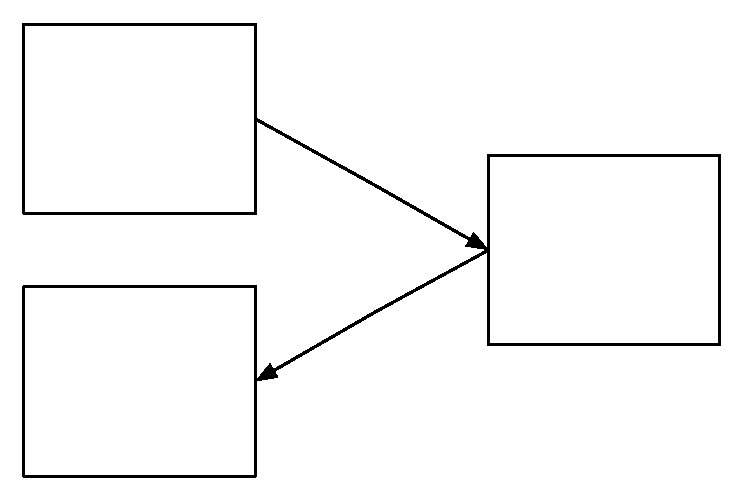
\includegraphics[width=0.5\columnwidth]{figs/figure1.pdf}
\caption[Boxes and arrows are nice]{Boxes and arrows are nice (adapted from \citet{authorson10:_secon_best_paper_in_world})}
\label{fig:BoxesAndArrowsAreNice}
\end{center}
\end{figure}

Remember that when you borrow figures you should always credit the original author --- such as Figure \ref{fig:BoxesAndArrowsAreNice} (adapted from \citet{authorson10:_secon_best_paper_in_world}). Also don't just put the figure in and leave it to the author to try to understand what the figure is. The figure should be put in to convey a message and you need to help the author to understand the message intended by explaining the figure in the text. 

\vspace{0.5cm}

\noindent
{\bf Introducing tables in the report: }\\

\begin{table}[htbp]
\begin{center}
\begin{tabular}{|c|c|c|c|c|}\hline\hline
This & is & a & nice & table\\\hline
This & is & a & nice & table\\\hline\hline
\end{tabular}
\caption{Example Table}
\end{center}
\label{tab:ExampleTable}
\end{table}%

As you can see from Table \ref{tab:ExampleTable}, tables are nice. However, again, you need to discuss the contents of the table in the text. You don't need to describe every entry but draw the authors attention to what is important for he/she to glean from the table. 
\fi

\iffalse
Here you need to include your structured review protocol including search engine, search words, research questions  (for search, not the masters research questions), inclusion createrias and evaluation Criterias. 
\fi

\iffalse
Your motivation can be either application driven or technique/methodology driven. However in both cases, there will be an element of methodology driven due to the research focus of our group and the nature of a masters project.  
What other research has been conducted in this area and how is it related to your work? The text should clearly illustrate why your goals and research questions are important to address. This section is thus where your literate review will be presented. It is important when presenting the review that you present an overview of the motivating elements of the work going on in your field and how these relate to your proposal, rather than a list of contributors and what they have done. This means that you need to extract the key important factors for your work and discuss how others have addressed each of these factors and what the advantages/disadvantages are with such approaches. As you mention other authors, you should reference their work. Note that the reference list reflects the literature you have read and have cited. This will only be a subset of the literature that you have read.
\fi
